\section{System Designs}
In this section, all of the design aspects of this system have been detailed and justified. This includes the design of the user interface itself, the navigation and expected user path through the application, and the internal design of the application.

\subsection{User Interface Design}
In this section, the interface for each of the main pages of the application have been displayed, along with justifications for why they were designed the way they were. Before any work was completed on the project, designs for each of these pages were produced, and shared with the client. The finale designs were then based on his feedback, and the combination of the best features from all the designs produced. These initial designs can be found in {\color{red} appendix A} and are referenced throughout this section.

\paragraph{Route Discovery Page/Landing Page}\ \\
\begin{figure}[!ht]
	\vspace{-5mm}
	\begin{center}
		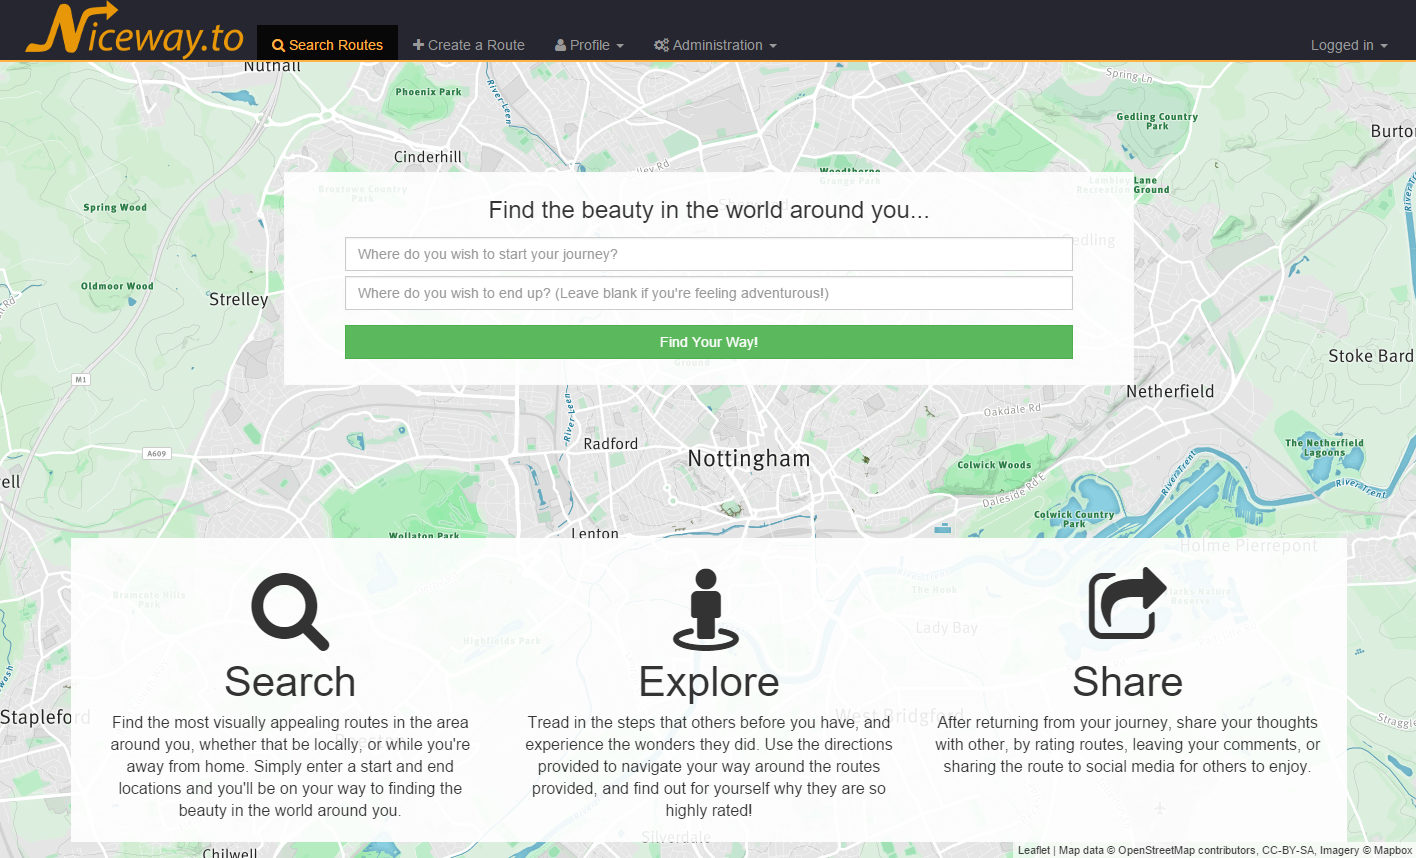
\includegraphics[width=0.8\textwidth]{images/design/landing.png}
	\end{center}
	\vspace{-5mm}
\end{figure}

{\color{red}
\noindent 
Why it is good\ \\
What was taken from each of the designs in the appendix\ \\
How it addresses the problem \ \\
Why it is designed the way it is\ \\
What differences there are to the designs
}

\paragraph{Route Listing Page}\ \\
\begin{figure}[!ht]
	\vspace{-5mm}
	\begin{center}
		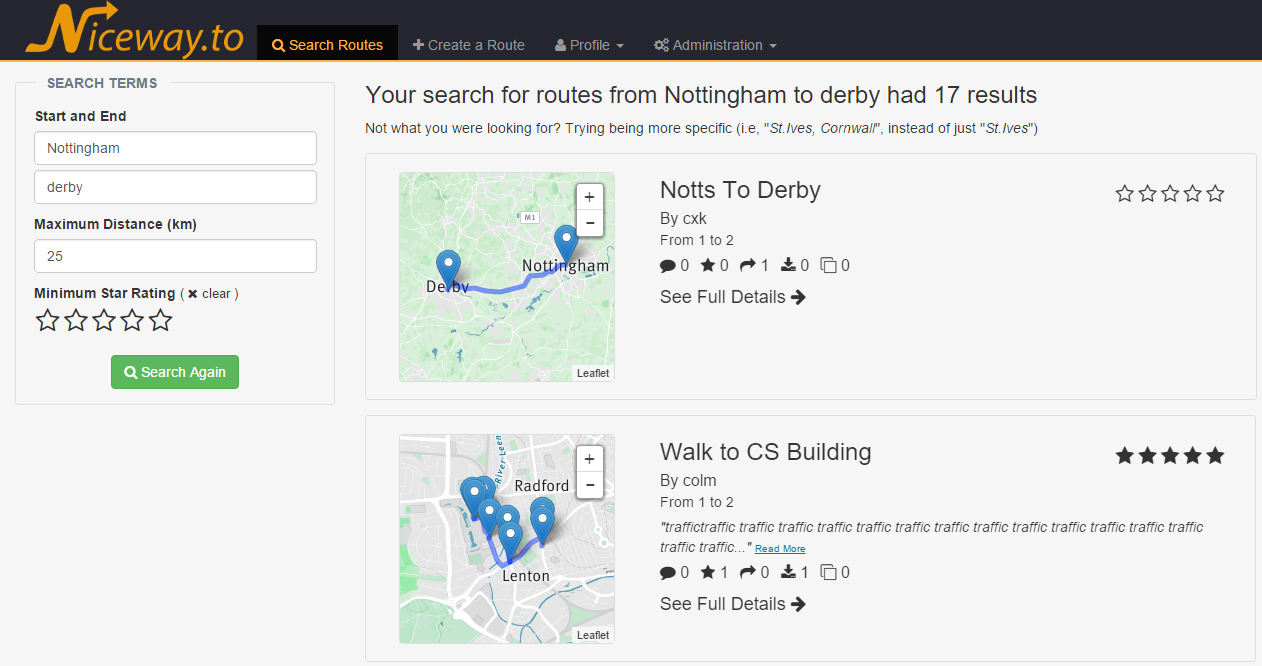
\includegraphics[width=0.5\textwidth]{images/design/listing.png}
	\end{center}
	\vspace{-10mm}
\end{figure}

{\color{red}
\noindent 
Why it is good\ \\
What was taken from each of the designs in the appendix\ \\
How it addresses the problem \ \\
Why it is designed the way it is\ \\
What differences there are to the designs
}

\newpage 
\paragraph{Route Detail Page}\ \\
\begin{figure}[!ht]
	\vspace{-5mm}
	\begin{center}
		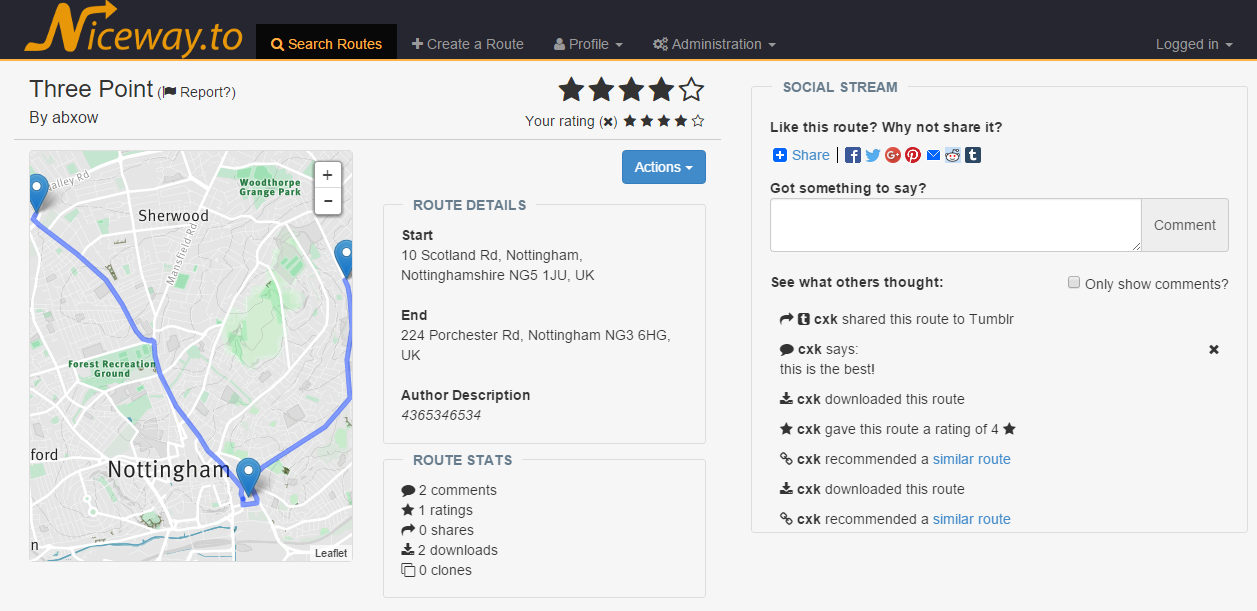
\includegraphics[width=0.7\textwidth]{images/design/detail.png}
	\end{center}
	\vspace{-5mm}
\end{figure}

{\color{red}
\noindent 
Why it is good\ \\
What was taken from each of the designs in the appendix\ \\
How it addresses the problem \ \\
Why it is designed the way it is\ \\
What differences there are to the designs
}

\paragraph{Route Creation Page}\ \\
\begin{figure}[!ht]
	\vspace{-5mm}
	\begin{center}
		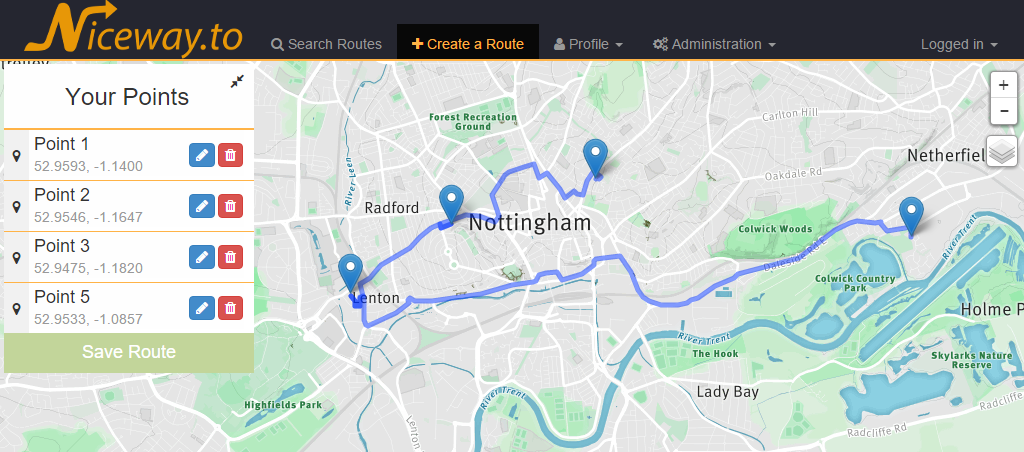
\includegraphics[width=0.7\textwidth]{images/design/create.png}
	\end{center}
	\vspace{-5mm}
\end{figure}

{\color{red}
\noindent 
Why it is good\ \\
What was taken from each of the designs in the appendix\ \\
How it addresses the problem \ \\
Why it is designed the way it is\ \\
What differences there are to the designs
}
{\color{blue} main client feedback was more social - so implemented the social stream to emphasize}

\paragraph{My Account Page}\ \\
\begin{figure}[!ht]
	\vspace{-5mm}
	\begin{center}
		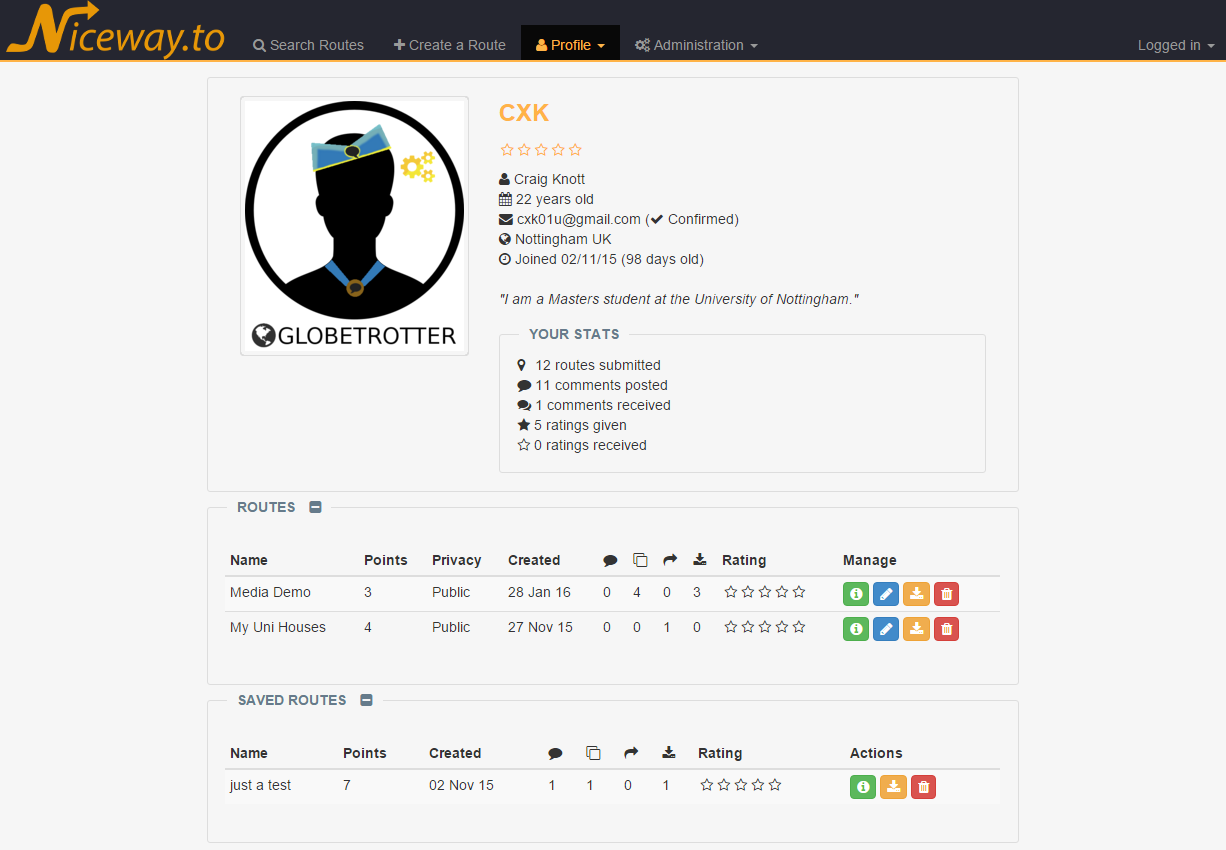
\includegraphics[width=0.5\textwidth]{images/design/profile.png}
	\end{center}
	\vspace{-5mm}
\end{figure}

{\color{red}
\noindent 
Why it is good\ \\
What was taken from each of the designs in the appendix\ \\
How it addresses the problem \ \\
Why it is designed the way it is\ \\
What differences there are to the designs
}

 
{\color{red}
Mention the magic number seven / white space is not your enemy stuff
White Space is Not Your Enemy: \cite{golombisky2013white}\ \\
The magical number seven, plus or minus two: \cite{miller1956magical}
Could I have the menu please? An eye tracking study of design conventions \cite{mccarthy2004could} - how navigation and elements on the page generally start on the left because that's where people (in western culture at least) will look first
Colour appeal in website design within and across cultures: A multi-method evaluation  \cite{cyr2010colour} - how colours have been used to group actions - green is pos, red is neg
Interface design technique to simplify and declutter your interfaces \cite{depot2014clutter} - icons, placeholders, controls on demand, hovers and modals
Satisfiers and Dissatisfiers: A Two-Factor Model for Website Design and Evaluation \cite{zhang2000satisfiers} - maybe this too...
}

\subsubsection{Heuristic Evaluation of the Interface}
In this section, the user interface is evaluated using several key metrics. These include: the general purpose usability heuristics identified by Jakob Nielsen\cite{nielsen199510}, the golden rules of interface design identified by Ben Schneiderman\cite{shneiderman2005designing}, and some heuristics specifically for the design of interfaces on mobiles device, identified by Nadav Savio\cite{savio2007design}. The purpose of this section is to highlight how the interface conforms to these metrics, and why they are important within the context of the application.\ \\
\ \\
{\color{red}
JN10: Visibility of system status\ \\
JN10: Match between system and the real world\ \\
JN10: User control and freedom\ \\
JN10: Consistency and standards\ \\
JN10: Error prevention\ \\
JN10: Recognition rather than recall\ \\
JN10: Flexibility and efficiency of use\ \\
JN10: Aesthetic and minimalist design\ \\
JN10: Help users recognize, diagnose, and recover from errors\ \\
JN10: Help and documentation\ \\
\ \\
BS8: Strive for consistency.\ \\
BS8: Cater to universal usability.\ \\
BS8: Offer informative feedback.\ \\
BS8: Design dialogs to yield closure.\ \\
BS8: Prevent errors.\ \\
BS8: Permit easy reversal of actions.\ \\
BS8: Support internal locus of control.\ \\
BS8: Reduce short-term memory load.\ \\
\ \\
MH10: All mobile interactions are user-driven. \ \\
MH10: New mobile experiences compete with legacy user models.  \ \\
MH10: Ease of use is paramount.  \ \\
MH10: Calm technology will be valued over constant disruptions.  \ \\
MH10: The device as continuous companion opens the realm for mobile experiences of different intensities and durations.  \ \\
MH10: Mobile interactions can extend beyond the device. \ \\
MH10: Mobile interactions are often small steps in part of larger user goals.  \ \\
MH10: Peer-to-peer is the most trusted form of mobile marketing.  \ \\
MH10: With GPS on the near horizon, the mobile phone will be able to provide services that redefine our social networks and the places we inhabit.  \ \\
MH10: Mobile phones will not be limited to the processing capabilities of the device. \ \\
}


\subsection{Navigation/Control Flow Design}
{\color{blue}
general path for non user - landing page (want to search, so box is very visible, like google), then results (clearly laid out results with ability to research if mistakes), and then detail page (display everything about the route, but ability to look deeper if user so wishes)\ \\
\ \\
general path for expert - login in, look at my account, check out new social interactions on their routes, look at friends routes, create a new route, update skins
}
{\color{red}
	\begin{itemize}
		\item The generally expected path for a user to take through the system + picture
		\item include path for both types of users
		\item Explain how design facilitates this - navigation for random access (except RLP)
	\end{itemize}
}

\subsection{Internal Design}
{\color{red}
	\begin{itemize}
		\item Models/Controller/Views with flow of data (plus ajax arc) (Mention client server stuff (probs in that diagram))
		\item Languages?
		\item See image from last year diss
	\end{itemize}
}


